\documentclass[12pt]{article}
\usepackage[utf8]{inputenc}
\usepackage{amsmath}
\usepackage{amssymb}
\usepackage{mathtools}
\usepackage{amsfonts}
\usepackage{lastpage}
\usepackage{tikz}
\usetikzlibrary{patterns}
\usepackage{pdfpages}
\usepackage{gauss}
\usepackage{fancyvrb}
\usepackage{fancyhdr}
\usepackage{graphicx}
\usepackage[margin=2.5 cm]{geometry}
\pagestyle{fancy}
\def\checkmark{\tikz\fill[scale=0.4](0,.35) -- (.25,0) -- (1,.7) -- (.25,.15) -- cycle;} 
\cfoot{Page \thepage\ of \pageref{LastPage}}
\DeclareGraphicsExtensions{.pdf,.png,.jpg}
\author{Nikolaj Dybdahl Rathcke (rfq695)}
\title{Første Aflevering \\ OR1}
\lhead{Nikolaj Dybdahl Rathcke (rfq695)}
\chead{OR1}
\rhead{Første aflevering}

\begin{document}
\maketitle
\section*{Opgave 1}
\subsection*{a}
Vi lader $x_1$ være antal $100$ liter vin og $x_2$ være antal $100$ liter øl og skriver da $P$ som.
\begin{equation}
\begin{array}{rrrrrl}
&\text{Max: } & -x_1 &- &2x_2 & \\
\hline
&\text{u.b.} &x_1 & & &\leq 2 \\
& & & &-x_2 &\leq -\frac{1}{2} \\
& &-x_1 &- &x_2 &\leq -\frac{5}{2} \\
& & & &x_1,x_2 &\geq 0
\end{array}
\end{equation}
Hvor vi vil maksimere den negative objektfunktion da det er et minimerings problem. Vi har desuden multipliceret nogle af bibetingelser med $-1$ så problemet er på standard form.

\subsection*{b}
Det duale problem bliver da
\begin{equation}
\begin{array}{rrrrrrrl}
&\text{Min: } &\xi=2y_1 &- &\frac{1}{2}y_2 &- &\frac{5}{2}y_3 & \\
\hline
&\text{u.b. } &y_1 & & &- &y_3 &\geq -1 \\
& & &- &y_2 &- &y_3 &\geq -2 \\
& & & & & &y_1,y_2,y_3 &\geq 0
\end{array}
\end{equation}
\newpage
\subsection*{c}
Her er problemet, $P$, skitseret
\begin{center}
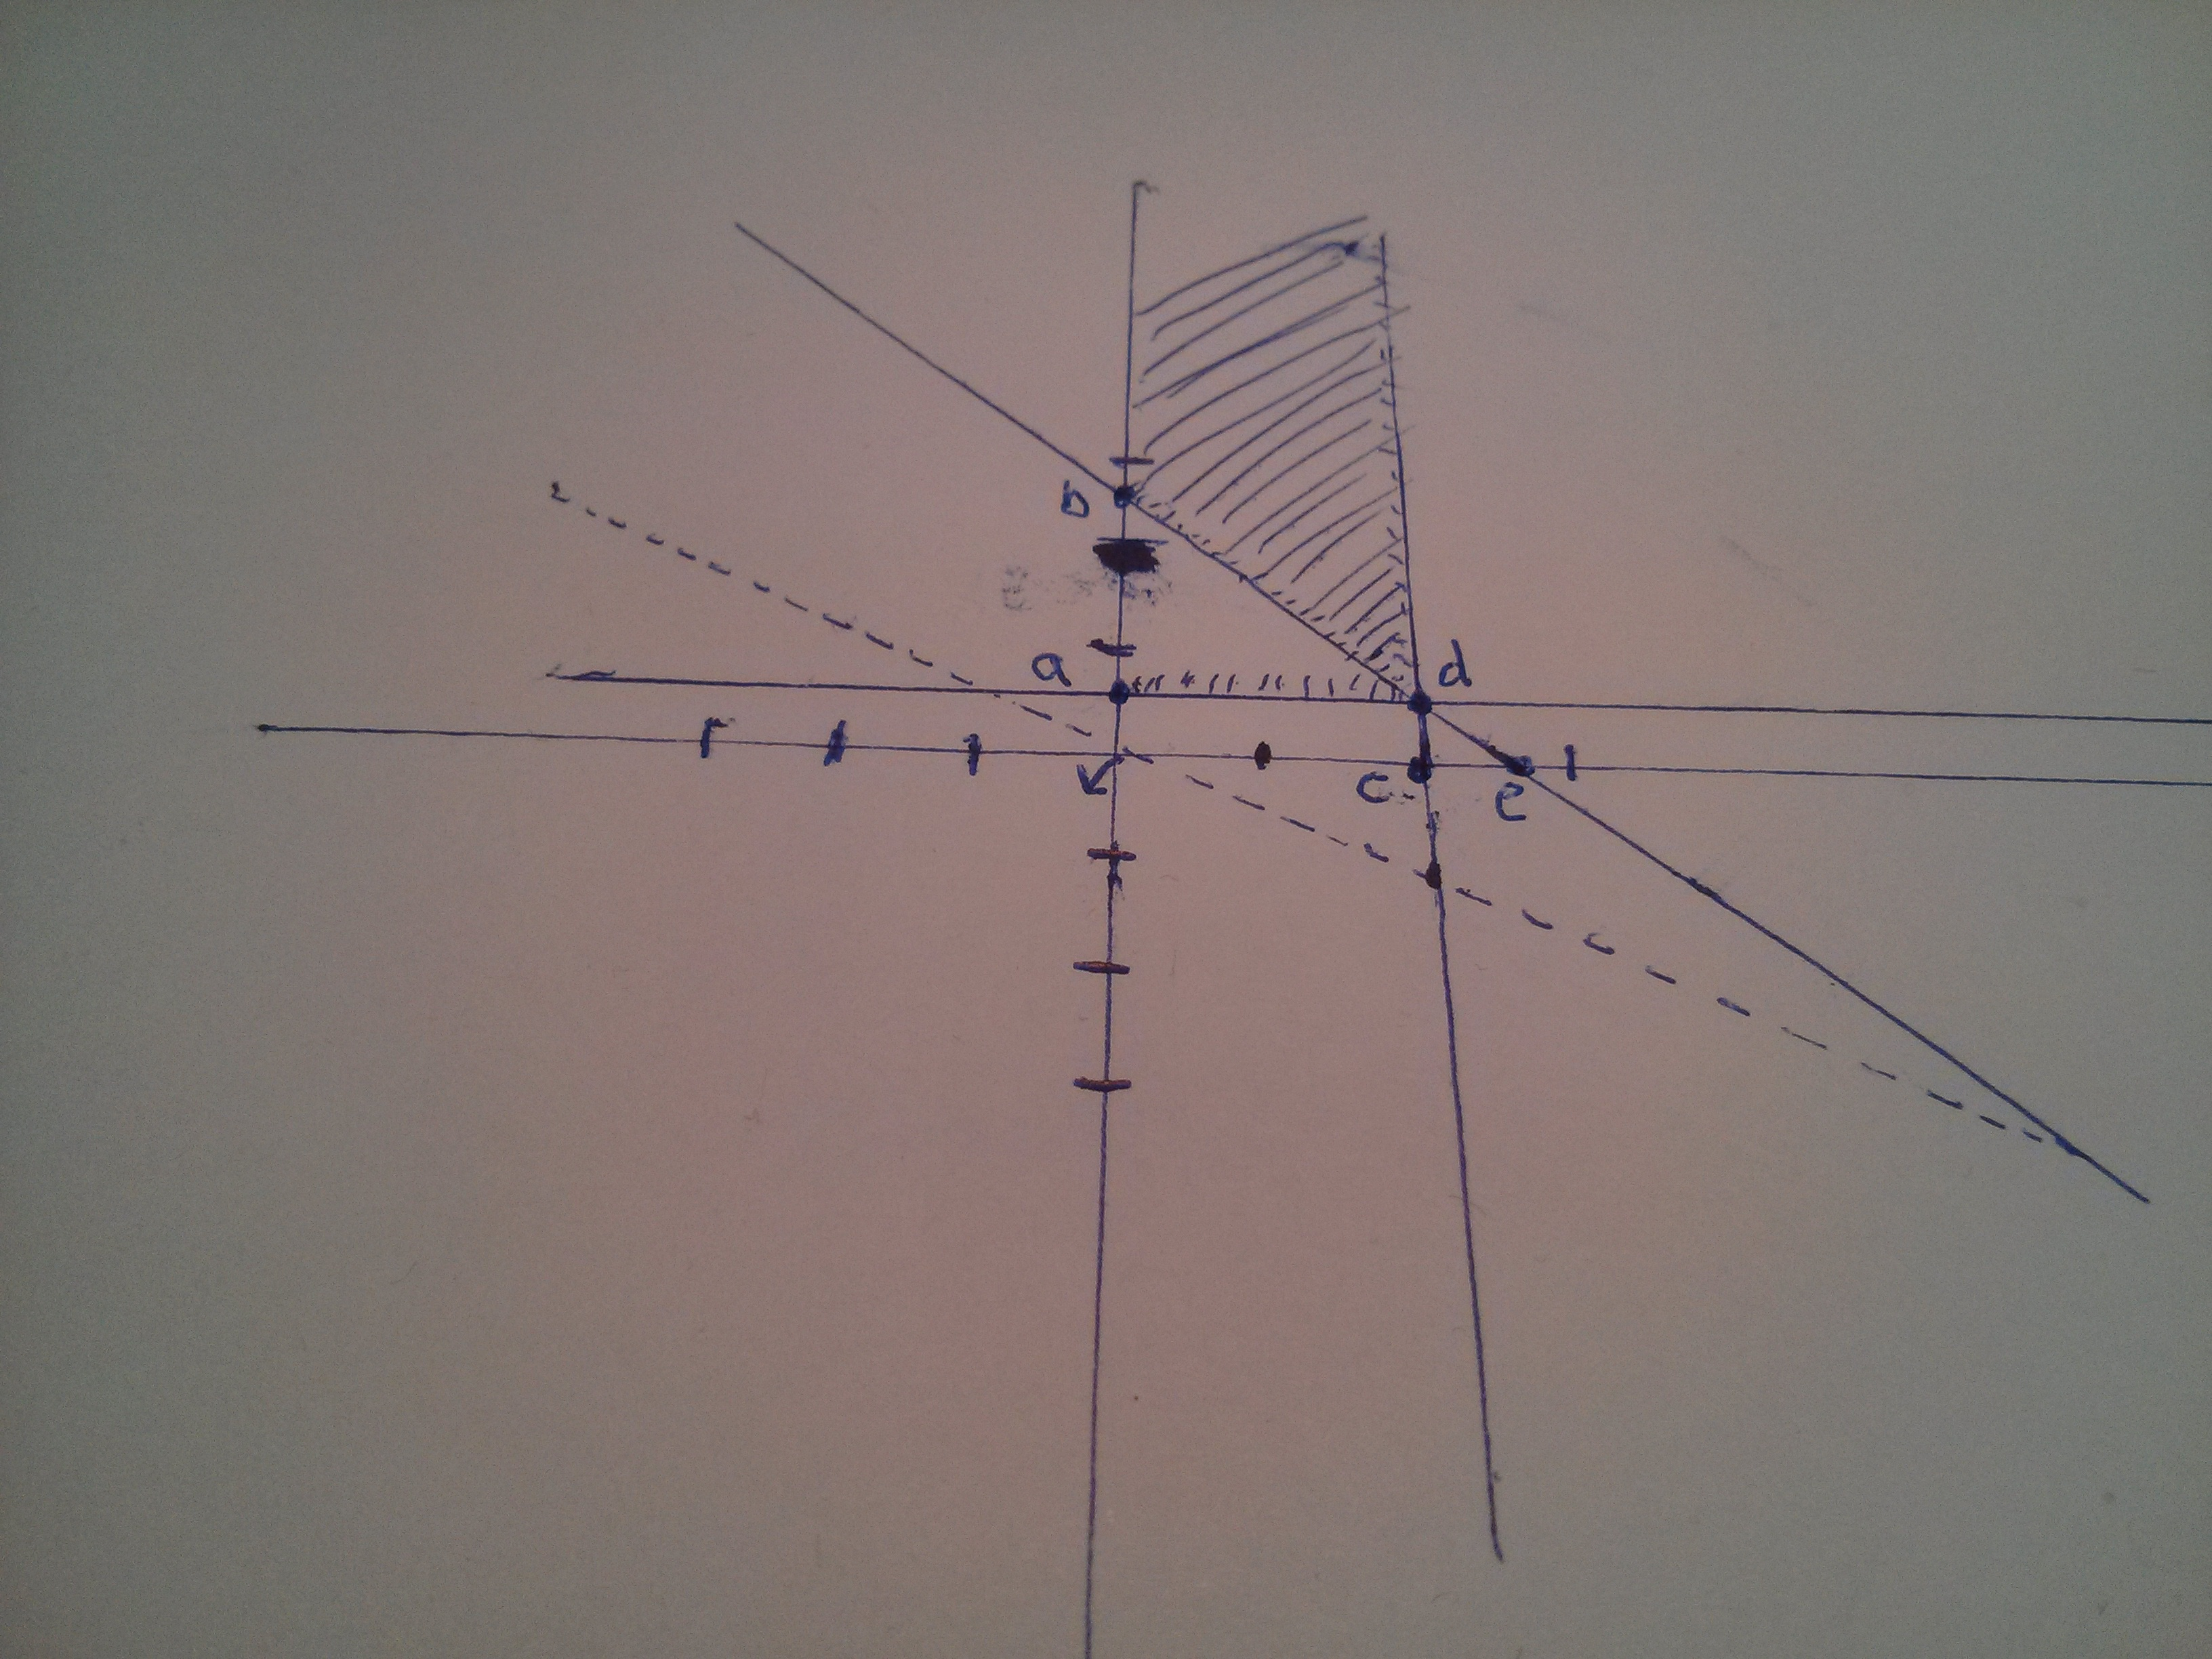
\includegraphics[scale=0.1]{1}
\end{center}
Hvor den stiplede linje er object funktionen.

\subsection*{d}
Først omskriver vi $P$ med slackvariablene $w_i$.
\begin{equation}
\begin{array}{rrrrrrrl}
&\text{Max: } & -x_1 &- &2x_2 & \\
\hline
&\text{u.b.} &x_1 & & & + &w_1&= 2 \\
& & & &-x_2 &+ &w_2 &= -\frac{1}{2} \\
& &-x_1 &- &x_2 &+ &w_3 &= -\frac{5}{2} \\
& & &\multicolumn{4}{r} {x_1,x_2,w_1,w_2,w_3} &\geq 0
\end{array}
\end{equation}

Herefter skriver vi $D$ med slackvariablene $z_i$
\begin{equation}
\begin{array}{rrrrrrrrrl}
&\text{Min: } &\xi=2y_1 &- &\frac{1}{2}y_2 &- &\frac{5}{2}y_3 & \\
\hline
&\text{u.b. } &y_1 & & &- &y_3 &- &z_1 &= -1 \\
& & & &-y_2 &- &y_3 &- &z_2 &= -2 \\
& & & &\multicolumn{5}{r} {y_1,y_2,y_3,z_1,z_2} &\geq 0
\end{array}
\end{equation}

\subsection*{e}
Hvis vi observerer billedet fra (c), kan vi finde $(x,w)=(x_1,x_2,x_3,w_1,w_2)$ til
\begin{align*}
a&=\left(0,\frac{1}{2},2,0,-2\right) \\
b&=\left(0,\frac{5}{2},2,2,0\right) \\
c&=\left(2,0,0,-\frac{1}{2},-\frac{1}{2}\right) \\
d&=\left(2,\frac{1}{2},0,0,0\right) \\
e&=\left(\frac{5}{2},0,-\frac{1}{2},-\frac{1}{2},0\right)
\end{align*}
Ligeledes finder vi $(z,y)=(z_1,z_2,y_1,y_2,y_3)$ til
\begin{align*}
a&=\left(1,0,0,2,0\right) \\
b&=\left(-1,0,0,0,2\right) \\
c&=\left(0,2,-1,0,0\right) \\
d&=\left(0,0,1,0,2\right) \\
e&=\left(0,1,0,0,1\right)
\end{align*}

\subsection*{f}
Nedenfor ses et skema for om de er primtalt/dualt brugbare eller ej.\\
Punkterne $b$ og $c$ er primalt brugbare, og vi kan bestemme det optimale punkt da et af disse må være det. Vi ser værdien for punktet $b$ giver $-2\cdot\frac{5}{2}=-5$ og for $d$ får vi $-2\cdot 1-2\cdot\frac{1}{2}=-3$. Altså er $d$ optimalt. Desuden er $b$ dualt ubrugbar.\\
Nu skal vi finde ud af om punkterne $a,c,e$ er dualt brugbare. Fra opgave (e) ser vi at ingen af basis variablene er negative for $a$ og $e$, altså er de brugbare. Dog er der negative basis variable for $c$ og den er derfor ikke brugbar
\begin{center}
\begin{tabular}{|c|c|c|c|}
\hline 
Punkt & Primalt brugbar & Dualt brugbar & Optimal \\ 
\hline 
a & \% & \checkmark & \% \\ 
\hline 
b & \checkmark & \% & \% \\ 
\hline 
c & \% & \% & \% \\ 
\hline 
d & \checkmark & \checkmark & \checkmark \\ 
\hline 
e & \% & \checkmark & \% \\ 
\hline 
\end{tabular} 
\end{center}

\subsection*{g}
Eftersom punktet $d$ er den optimale funktion, ser vi, at $200$ liter vin og $50$ liter øl er optimalt og derfor billigst.

\section*{Opgave 2}
\subsection*{a}
Vi vil løse følgende hjælpeproblem med simplex metoden
\begin{equation}
\begin{array}{rrrrrrrl}
&\text{Max: } & -x_0 & & & & & \\
\hline
&\text{u.b.} &x_1 & & &- &x_0 &\leq 2 \\
& & & &-x_2 &- &x_0 &\leq -\frac{1}{2} \\
& &-x_1 &- &x_2 &- &x_0 &\leq -\frac{5}{2} \\
& & & &  \multicolumn{3}{r} {x_1,x_2,x_0} &\geq 0
\end{array}
\end{equation}
Vi starter med at tilføje slack variablene og får
\begin{equation}
\begin{array}{rrrrrrrrrl}
&\xi &= & & & & & & -&x_0 \\
\hline
&w_1 &= &2 &- &x_1 & & &+ &x_0 \\
&w_2 &= &-\frac{1}{2} & & &+ &x_2 &+ &x_0 \\
&w_3 &= &-\frac{5}{2} &+ &x_1 &+ &x_2 &+ &x_0 \\
\end{array}
\end{equation}
Indgående: $x_0$ \\
Udgående: $w_3$ \\
Isolering af $x_0$ i ligningen for $w_3$ giver
$$x_0=\frac{5}{2}-x_1-x_2+w_3$$
Dette giver os at $\xi,w_1$ og $w_2$ er
\begin{align*}
\xi&=-\frac{5}{2}+x_1+x_2+w_3 \\
w_1&=\frac{9}{2}-2x_1-x_2+w_3 \\
w_2&=2-x_1+w_3
\end{align*}
Dette giver os det nye tableau
\begin{equation}
\begin{array}{rrrrrrrrrl}
&\xi &= &-\frac{5}{2}&+&x_1&+&x_2&-&w_3\\
\hline
&w_1 &= &\frac{9}{2} &- &2x_1 &- &x_2 &+ &w_3 \\
&w_2 &= &2 &- &x_1 & & &+ &w_3 \\
&x_0 &= &\frac{5}{2} &- &x_1 &- &x_2 &+ &w_3 \\
\end{array}
\end{equation}
Indgående: $x_2$ \\
Ratio: $(-\frac{-1}{\frac{9}{2}},0,-\frac{-1}{\frac{5}{2}})=(\frac{2}{9},0,\frac{2}{5})$ \\
Max: $\frac{2}{5}$ \\
Udgående: $x_0$ \\
Isolering af $x_2$ i $x_0$ giver
$$x_2=\frac{5}{2}-x_1+w_3-x_0$$
Som giver os vores tredje tableau
\begin{equation}
\begin{array}{rrrrrrrrrrrl}
&\xi &= &-x_0&&&&&\\
\hline
&w_1 &= &2&-&x_1&&&+&x_0&&\\
&w_2&=&2&-&x_1&+&w_3&&&& \\
&x_2&=&\frac{5}{2}&-&x_1&+&w_3&+&x_0&&
\end{array}
\end{equation}
Variablen $x_0$ forsvinder da det er optimalt. Nu introducerer vi den originale object funktion og vi får følgende tableau.
\begin{equation}
\begin{array}{rrrrrrrrrrrl}
&\xi &= &-5&+&x_1&-&2w_3&&&\\
\hline
&w_1 &= &2&-&x_1&&&&&&\\
&w_2&=&2&-&x_1&+&w_3&&&& \\
&x_2&=&\frac{5}{2}&-&x_1&+&w_3&&&&
\end{array}
\end{equation}
Indgående: $x_1$ \\
Ratio: $(-\frac{-1}{2},-\frac{-1}{2},-\frac{-1}{\frac{5}{2}})=(\frac{1}{2},\frac{1}{2},\frac{2}{5})$ \\
Max: $\frac{1}{2}$ \\
Udgående: $w_1$ \\
Isolering af $x_1$ i $w_1$ giver
$$x_1=2-w_1$$
Som giver os følgende tableau
\begin{equation}
\begin{array}{rrrrrrrrrrrl}
&\xi &= &-3&-&w_1&-&2w_3&&&\\
\hline
&x_1 &= &2&-&w_1&&&&&&\\
&w_2&=&&&w_1&+&w_3&&&& \\
&x_2&=&\frac{1}{2}&+&w_1&+&w_3&&&&
\end{array}
\end{equation}
Nu er den optimal idet der kun er negative koefficient i objektfunktionen.


\subsection*{b}
Den gennemløb først punktet $b$ i (9) som lægger i $(0,\frac{5}{2})$ og herefter ramte den punktet $d$ (10) i $(2,\frac{1}{2})$.


\subsection*{c}
Nu løses det duale problem med simplex metoden.
\begin{equation}
\begin{array}{rrrrrrrl}
&\text{Min: } &\xi=2y_1 &- &\frac{1}{2}y_2 &- &\frac{5}{2}y_3 & \\
\hline
&\text{u.b. } &y_1 & & &- &y_3 &\geq -1 \\
& & &- &y_2 &- &y_3 &\geq -2 \\
& & & & & &y_1,y_2,y_3 &\geq 0
\end{array}
\end{equation}
Det skriver vi om så vi får
\begin{equation}
\begin{array}{rrrrrrrrrl}
&-\xi&=&-2y_1 &+ &\frac{1}{2}y_2 &+ &\frac{5}{2}y_3& \\
\hline
&z_1&=&1&+&y_1&&&-&y_3 \\
&z_2&=&2&&&-&y_2 &- &y_3  \\
\end{array}
\end{equation}
Indgående: $y_3$ \\
Ratio: $(-\frac{-1}{1},-\frac{-1}{2})=(1,\frac{1}{2})$ \\
Max: $1$ \\
Udgående: $z_1$ \\
Isolering af $y_3$ i $z_1$ giver
$$y_3=1+y_1-z_1$$
Som giver os følgende tableau
\begin{equation}
\begin{array}{rrrrrrrrrl}
&-\xi&=&\frac{5}{2}&+&\frac{1}{2}y_1 &+&\frac{1}{2}y_2&- &\frac{5}{2}z_1 \\
\hline
&y_3&=&1&+&y_1&&&-&z_1 \\
&z_2&=&1&-&y_1&-&y_2&+ &z_1  \\
\end{array}
\end{equation}
Indgående: $y_1$ \\
Ratio: $(-\frac{1}{1},-\frac{-1}{1})=(-1,1)$ \\
Max: $1$ \\
Udgående: $z_2$ \\
Isolering af $y_1$ i $z_2$ giver
$$y_1=1-y_2+z_1-z_2$$
Dette giver det næste tableau
\begin{equation}
\begin{array}{rrrrrrrrrl}
&-\xi&=&3&-&\frac{1}{2}z_1 &-&2z_2& & \\
\hline
&y_3&=&2&-&y_2&-&&&z_2 \\
&y_1&=&1&-&y_2&+&z_1&- &z_2  \\
\end{array}
\end{equation}
Og nu er den optimal.

\subsection*{d}
Den gennemløb punkt $e$ i (13) med $(z_1,z_2,y_1,y_2,y_3)=(0,1,0,0,1)$ samt punktet $d$ i (14) med $(z_1,z_2,y_1,y_2,y_3)=(0,0,1,0,2)$.

\subsection*{e}
Variablene $(x,w)$ kan aflæses fra skemaerne ved at kigge på konstanterne i rækkerne under objektfunktionen, så i (9) får vi at: $w_1=2,w_2=2$ og $x_2=\frac{5}{2}$ for punktet $b$. \\
Desuden kan variablene $(z,y)$ aflæses ud fra objektfunktionen hvor i vores tilfælde vi har $(x_1,x_2,w_1,w_2,w_3)=(z_1,z_2,y_1,y_2,y_3)$. Her er det koefficienterne negeret. Altså fra (9) får vi at $x_1=z_1=-1$ og $w_3=y_3=2$. \\
De variable der ikke indgår bliver sat til $0$ i begge tilfælde.

\subsection*{f}
Dette er egentligt bare det omvendte af (e). Så $(x,w)$ aflæses ved at kigge på objektfunktionen. I (13) har vi derfor at $y_1=w_1=-\frac{1}{2},y_2=w_2=-\frac{1}{2}$ og $z_1=x_1=\frac{5}{2}$ \\
Ligeledes har vi at $(z,y)$ i (13) er $(0,1,0,0,1)$ - aflæst direkte fra rækkerne.

\subsection*{g}
Det var lettest at løse $D$ idet der ikke var brug for et hjælpeproblem og derved var der færre iterationer.

\section*{Opgave 3}
\subsection*{a}
Eftersom dette svarer til en ændring af tredje begrænsning, $b_3$, fra $-x_1-2x_2\leq -\frac{5}{2}$ til $-x_1-2x_2\leq -5$ får vi at $\Delta b_3= -\frac{5}{2}-(-5)=\frac{5}{2}$. Idet vores optimale basis var $(1,0,2)$ må det betyde at vi får en ændring i vores objektfunktion på $\Delta b_3y_3=\frac{5}{2}\cdot 2=5$ - altså en objektværdi på $3+5=8$ da objektværdien var $3$ før. Dette gælder kun hvis \\

\subsection*{b}
2

\subsection*{c}
3



\end{document}

--------------------